

\section{Struttura delle classi}

\subsection{\texttt{quasylab.sibilla.core.network}}
Il package di riferimento relativo alla \textbf{libreria sviluppata}. Le classi contenute al suo interno hanno la natura di wrapper di dati e hanno un impiego condiviso da parte degli ulteriori pacchetti, ognuno presente con responsabilità e finalità definiti:

\begin{figure}[H]
  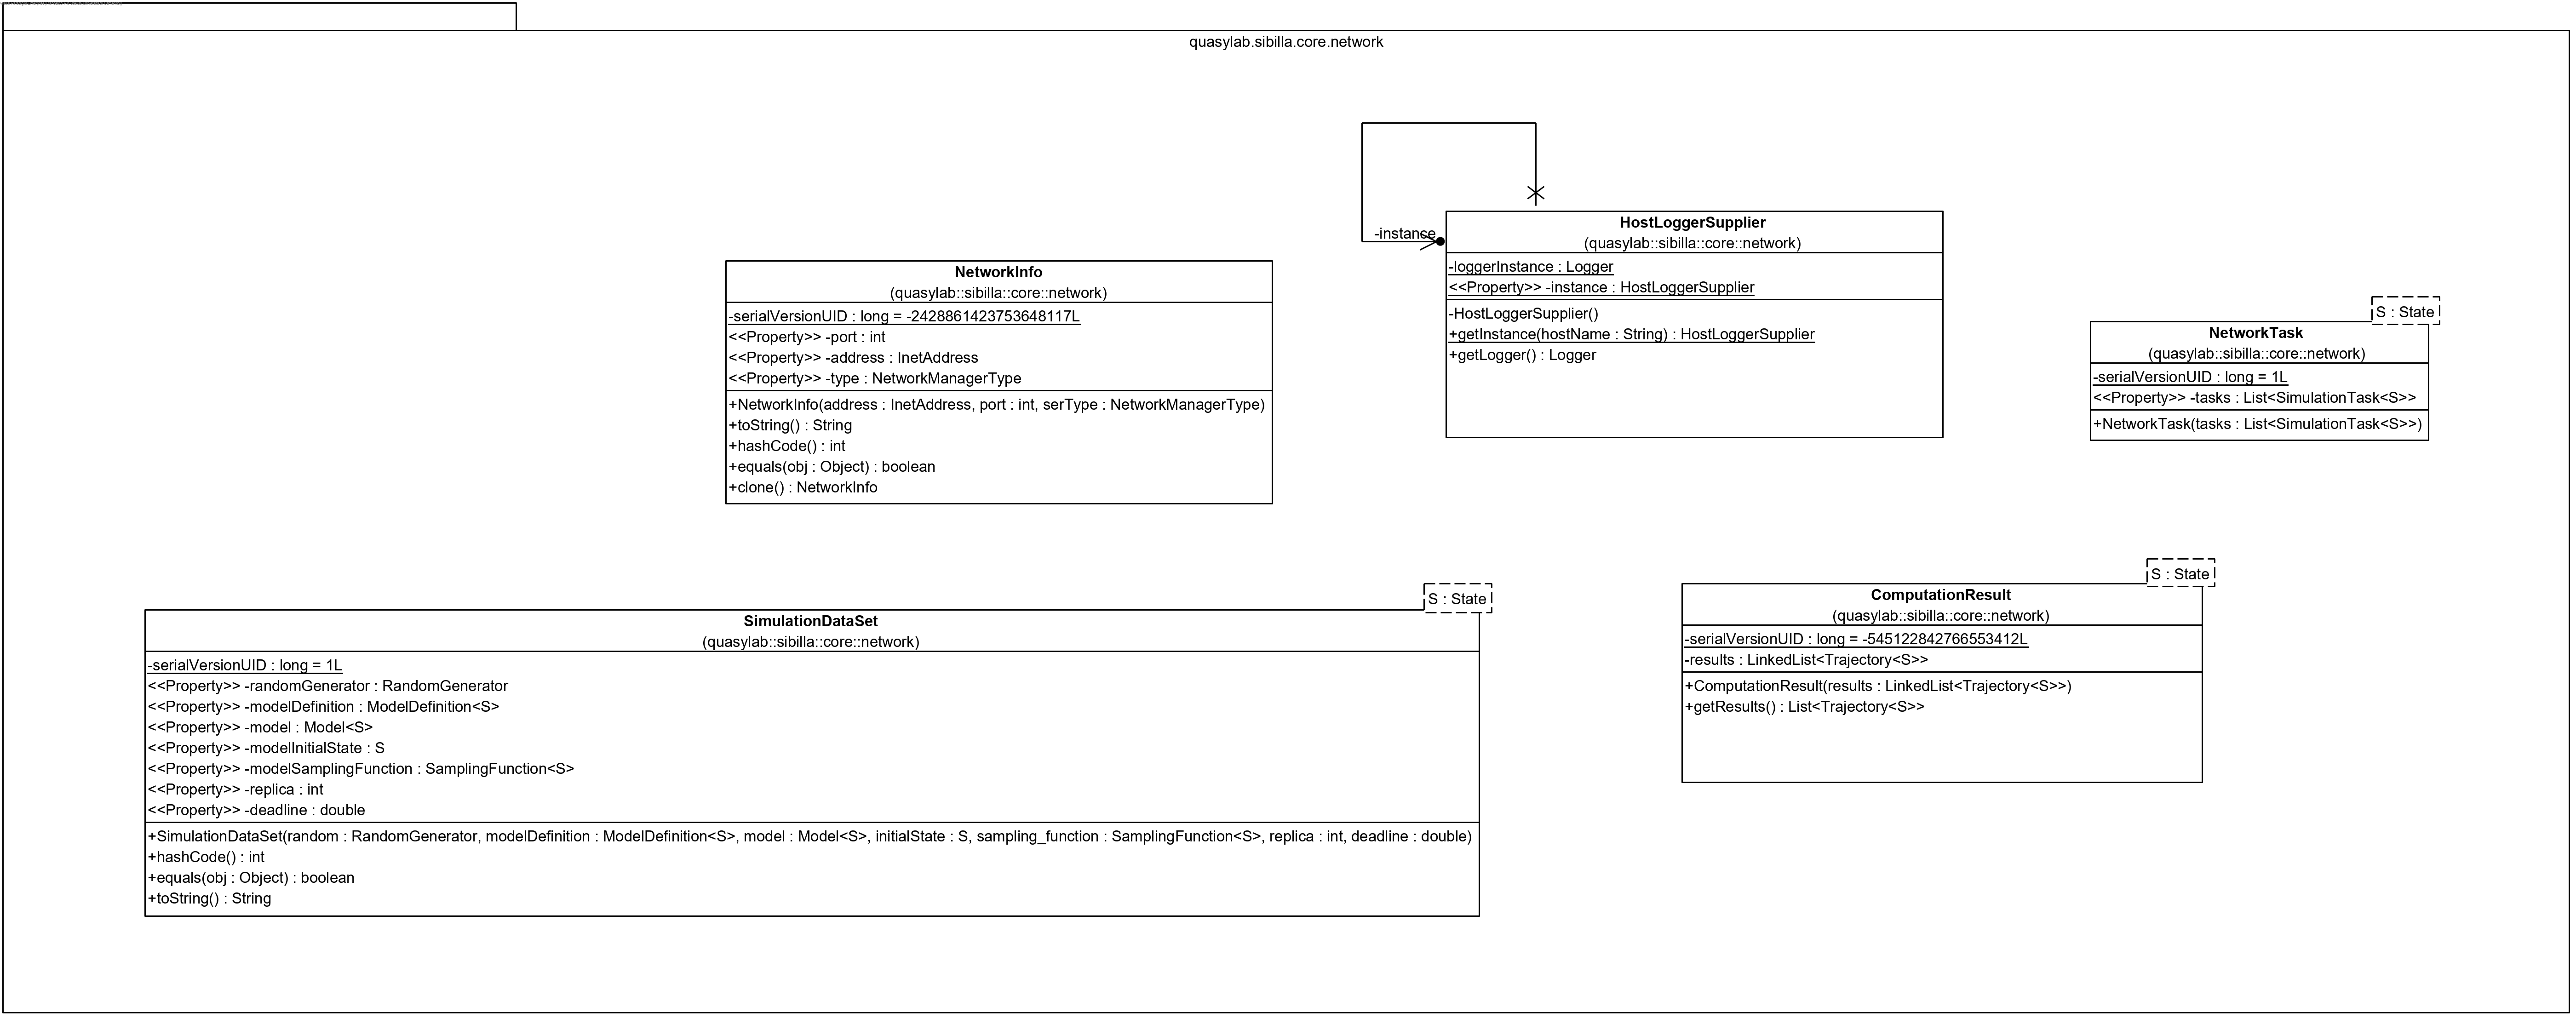
\includegraphics[width=\linewidth]{images/quasylab.sibilla.core.network.png}
  \captionsetup{justification=centering}
  \caption{Diagramma delle classi del package \texttt{quasylab.sibilla.core.network}}
\end{figure}

\subsection{\texttt{quasylab.sibilla.core.network.client}} Contiene tutte le classi utili a inizializzare un nuovo \textbf{client} e a gestire la comunicazione con un server master.

\begin{figure}[H]
    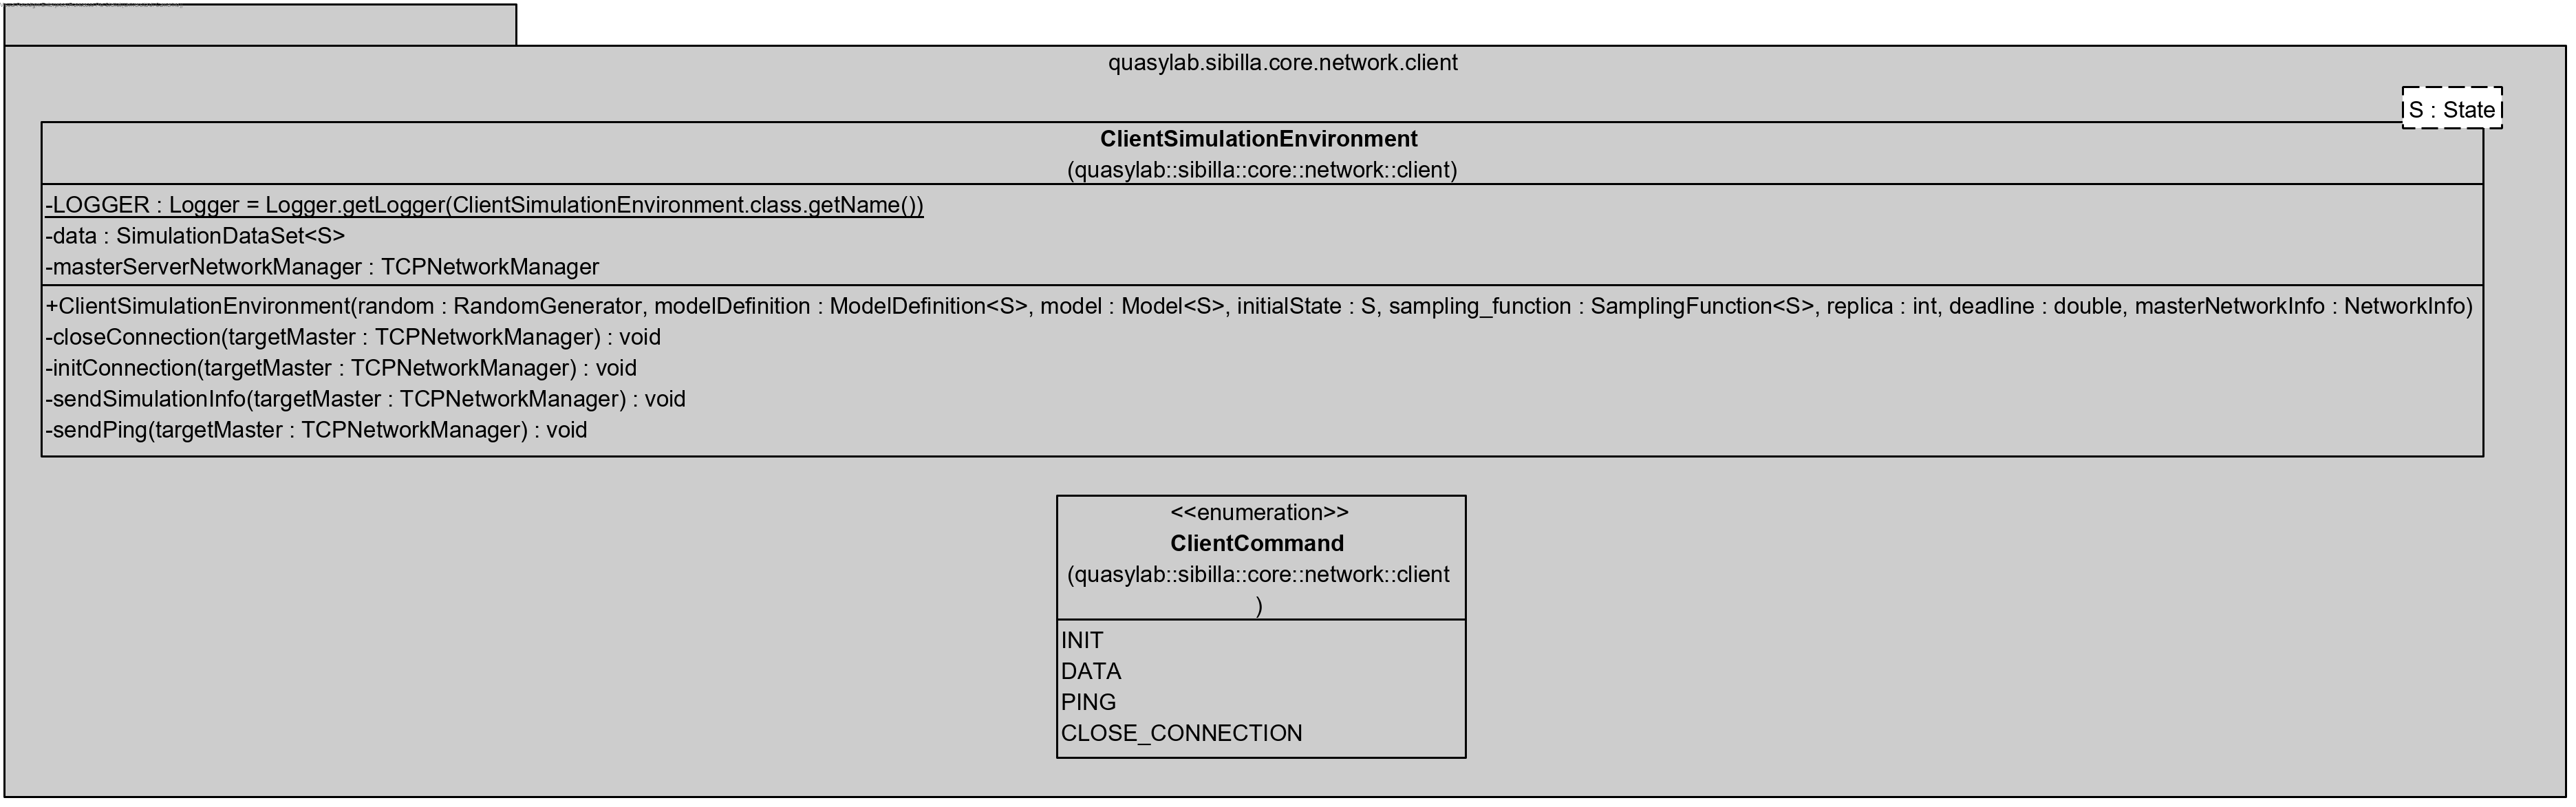
\includegraphics[width=\linewidth]{images/quasylab.sibilla.core.network.client.png}
    \captionsetup{justification=centering}
    \caption{Diagramma delle classi del package \texttt{quasylab.sibilla.core.network.client}}
  \end{figure}

\subsection{\texttt{quasylab.sibilla.core.network.master}} Contiene tutte le classi utili a inizializzare un nuovo \textbf{server master} e a gestire la comunicazione con tutti i client che sottomettono ad esso simulazione e con tutti i server slave che sono presenti all’interno della rete in cui tale master è avviato.

\begin{figure}[H]
    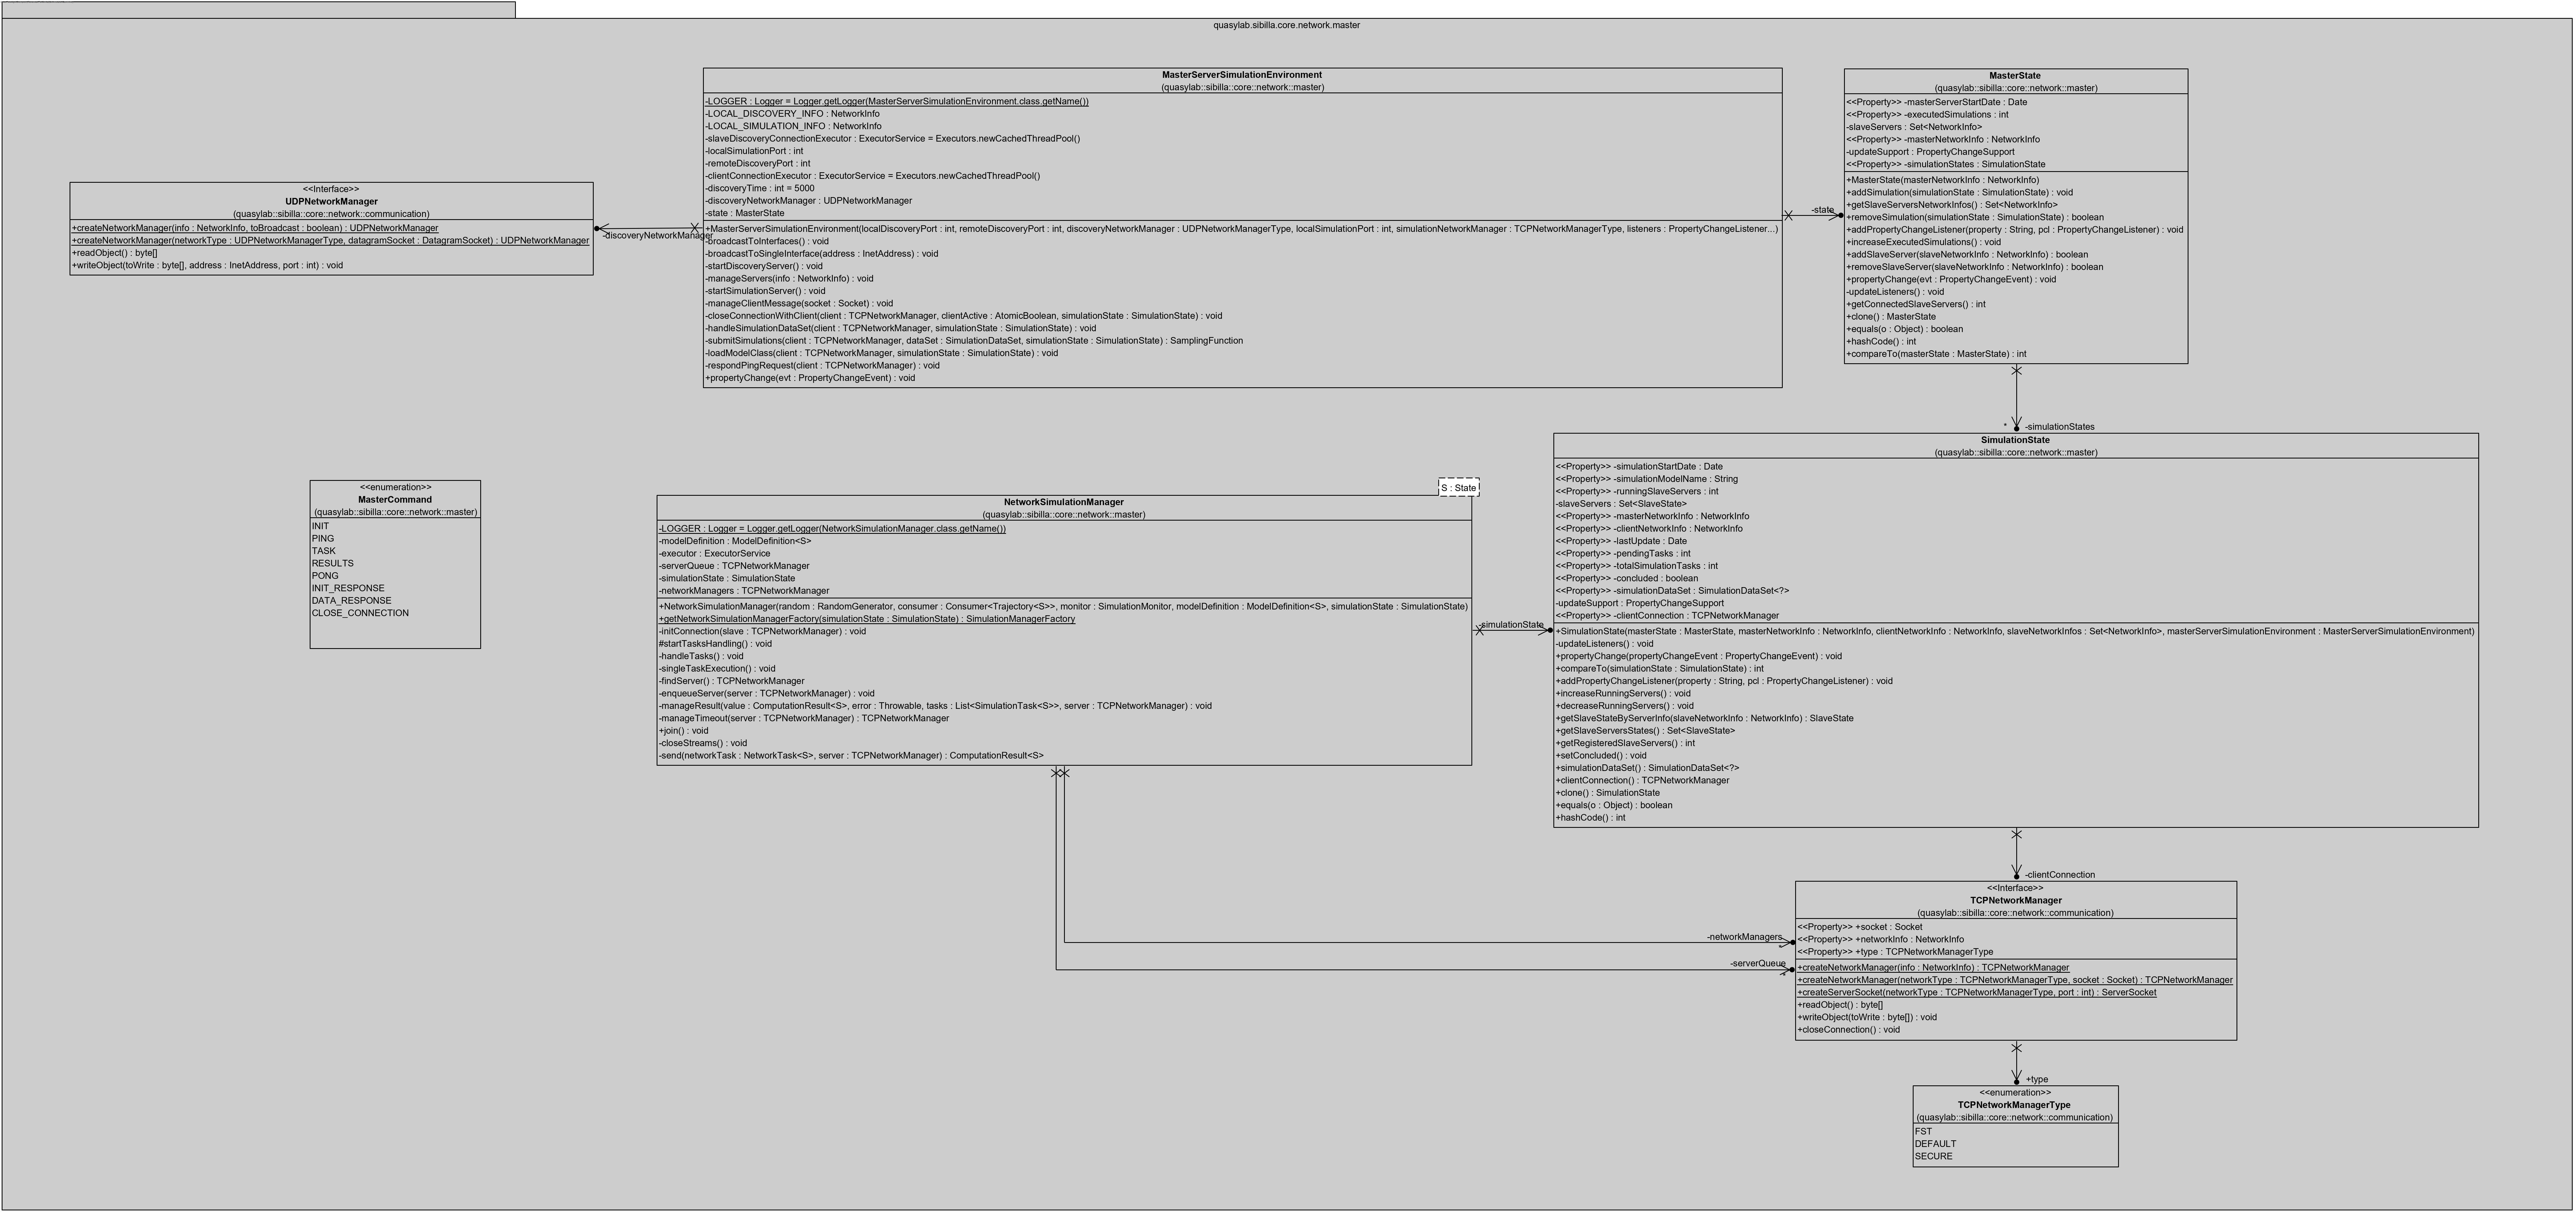
\includegraphics[width=\linewidth]{images/quasylab.sibilla.core.network.master.png}
    \captionsetup{justification=centering}
    \caption{Diagramma delle classi del package \texttt{quasylab.sibilla.core.network.master}}
  \end{figure}

\subsection{\texttt{quasylab.sibilla.core.network.slave}} Contiene tutte le classi utili a inizializzare un nuovo \textbf{server slave} e a gestire la comunicazione con tutti i server master che inviano messaggi di discovery e sottomettono simulazioni.

\begin{figure}[H]
    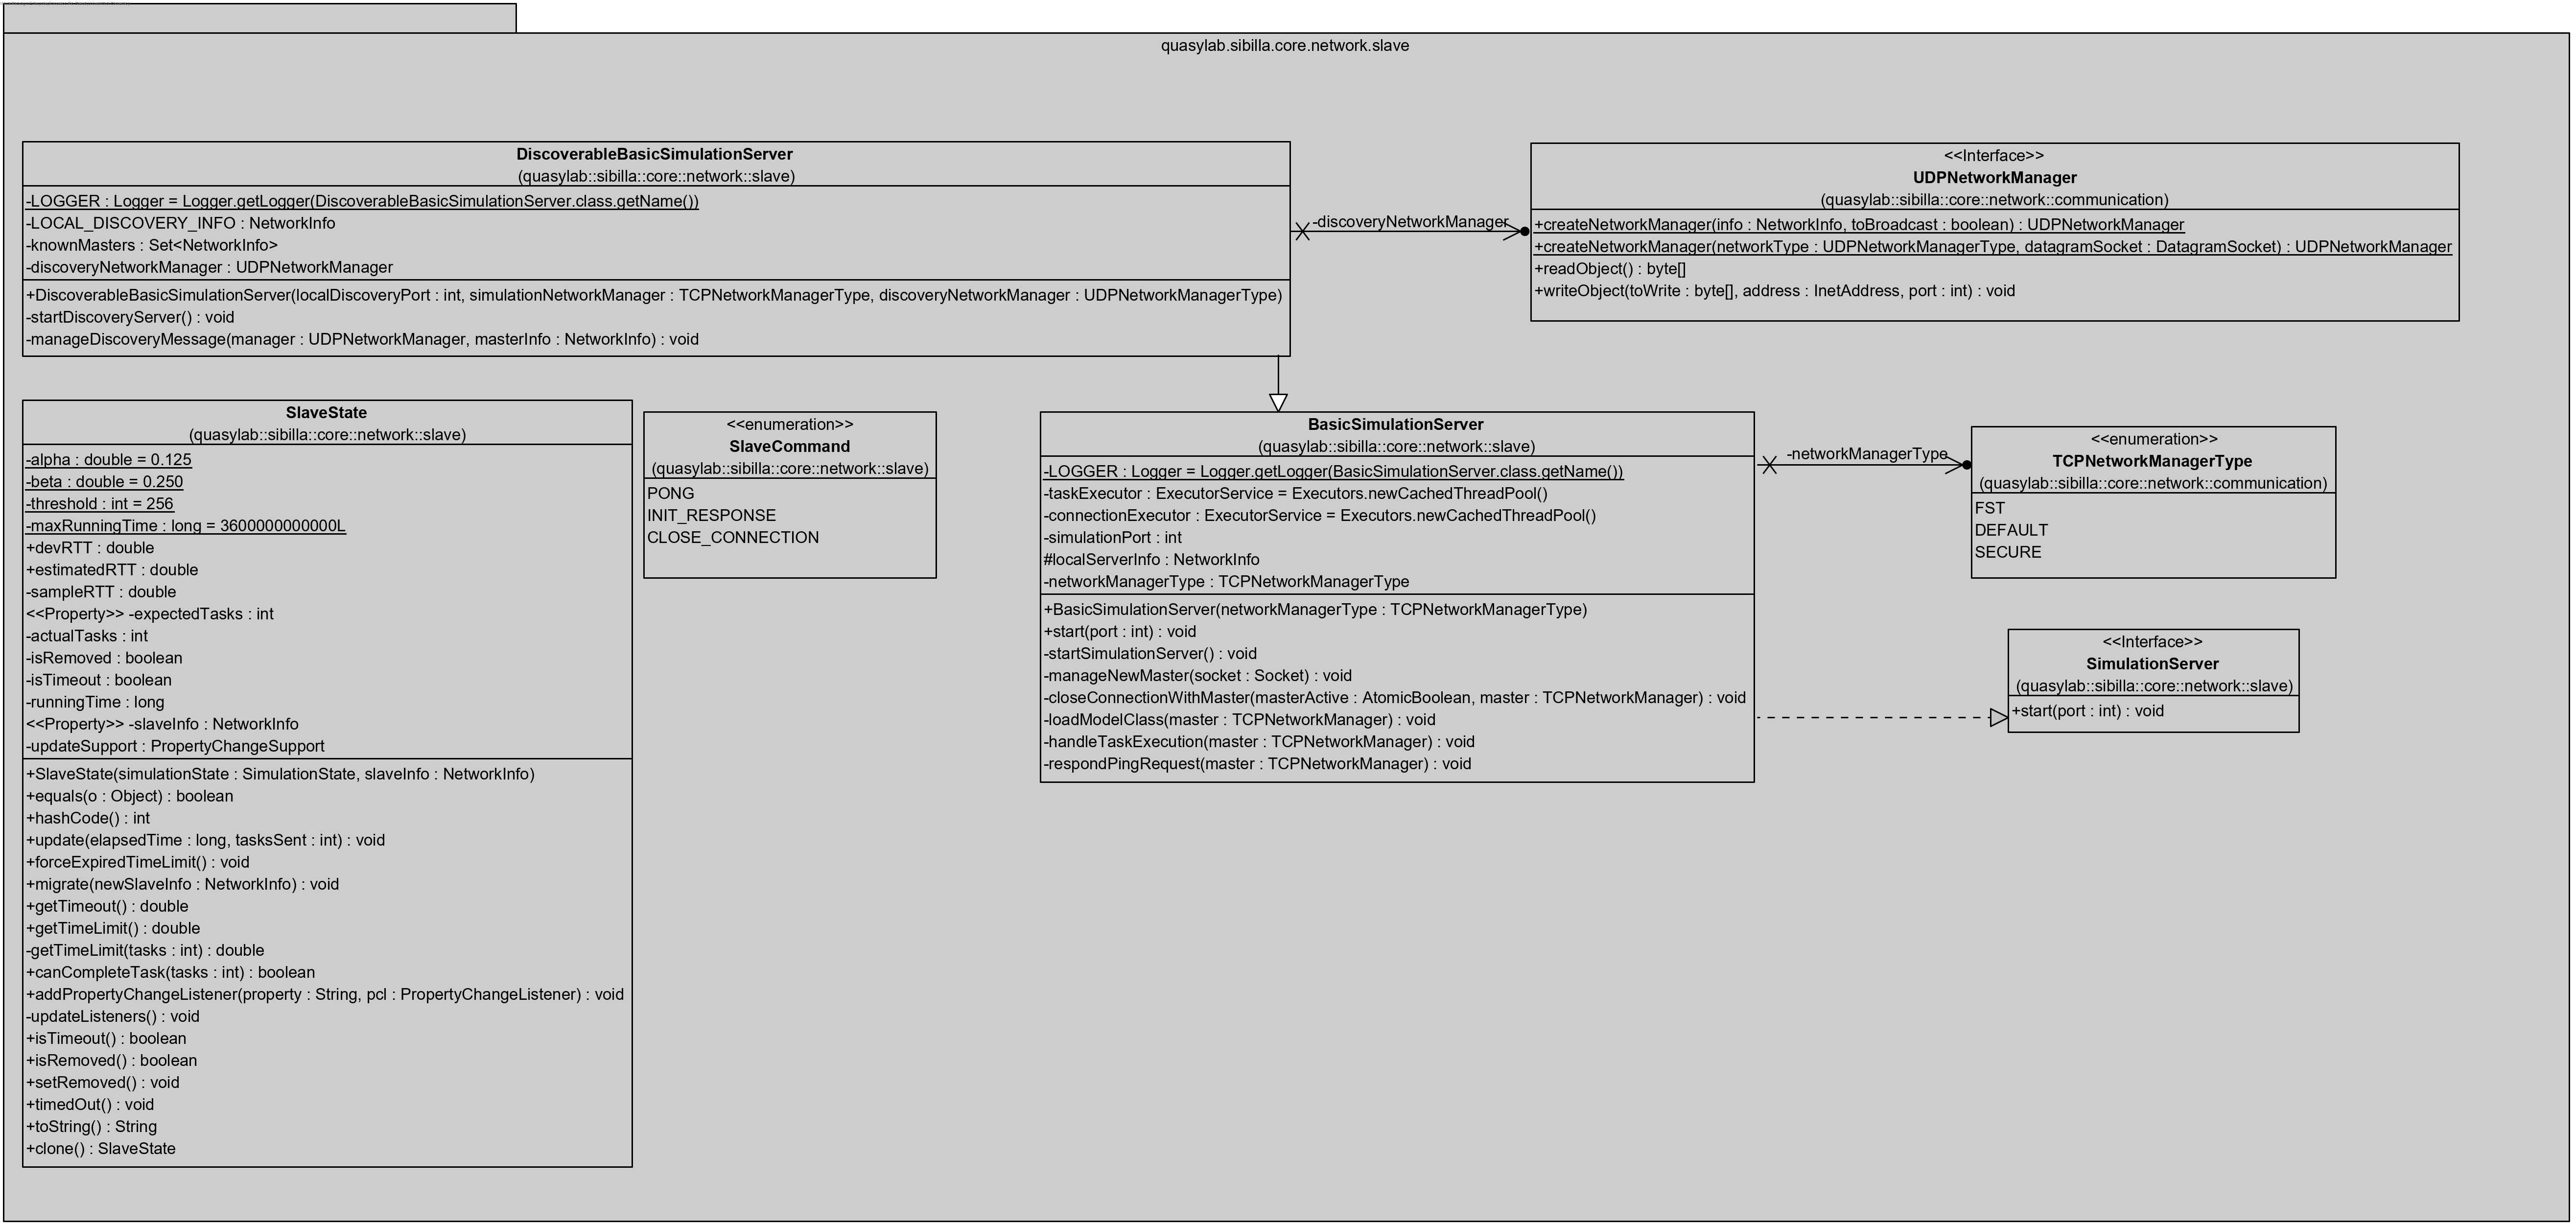
\includegraphics[width=\linewidth]{images/quasylab.sibilla.core.network.slave.png}
    \captionsetup{justification=centering}
    \caption{Diagramma delle classi del package \texttt{quasylab.sibilla.core.network.slave}}
  \end{figure}

\subsection{\texttt{quasylab.sibilla.core.network.communication}} Contiene le classi che si occupano di gestire la \textbf{comunicazione} tramite i vari nodi dell’infrastruttura basandosi sui protocolli di trasporto TCP e UDP. 

\begin{figure}[H]
    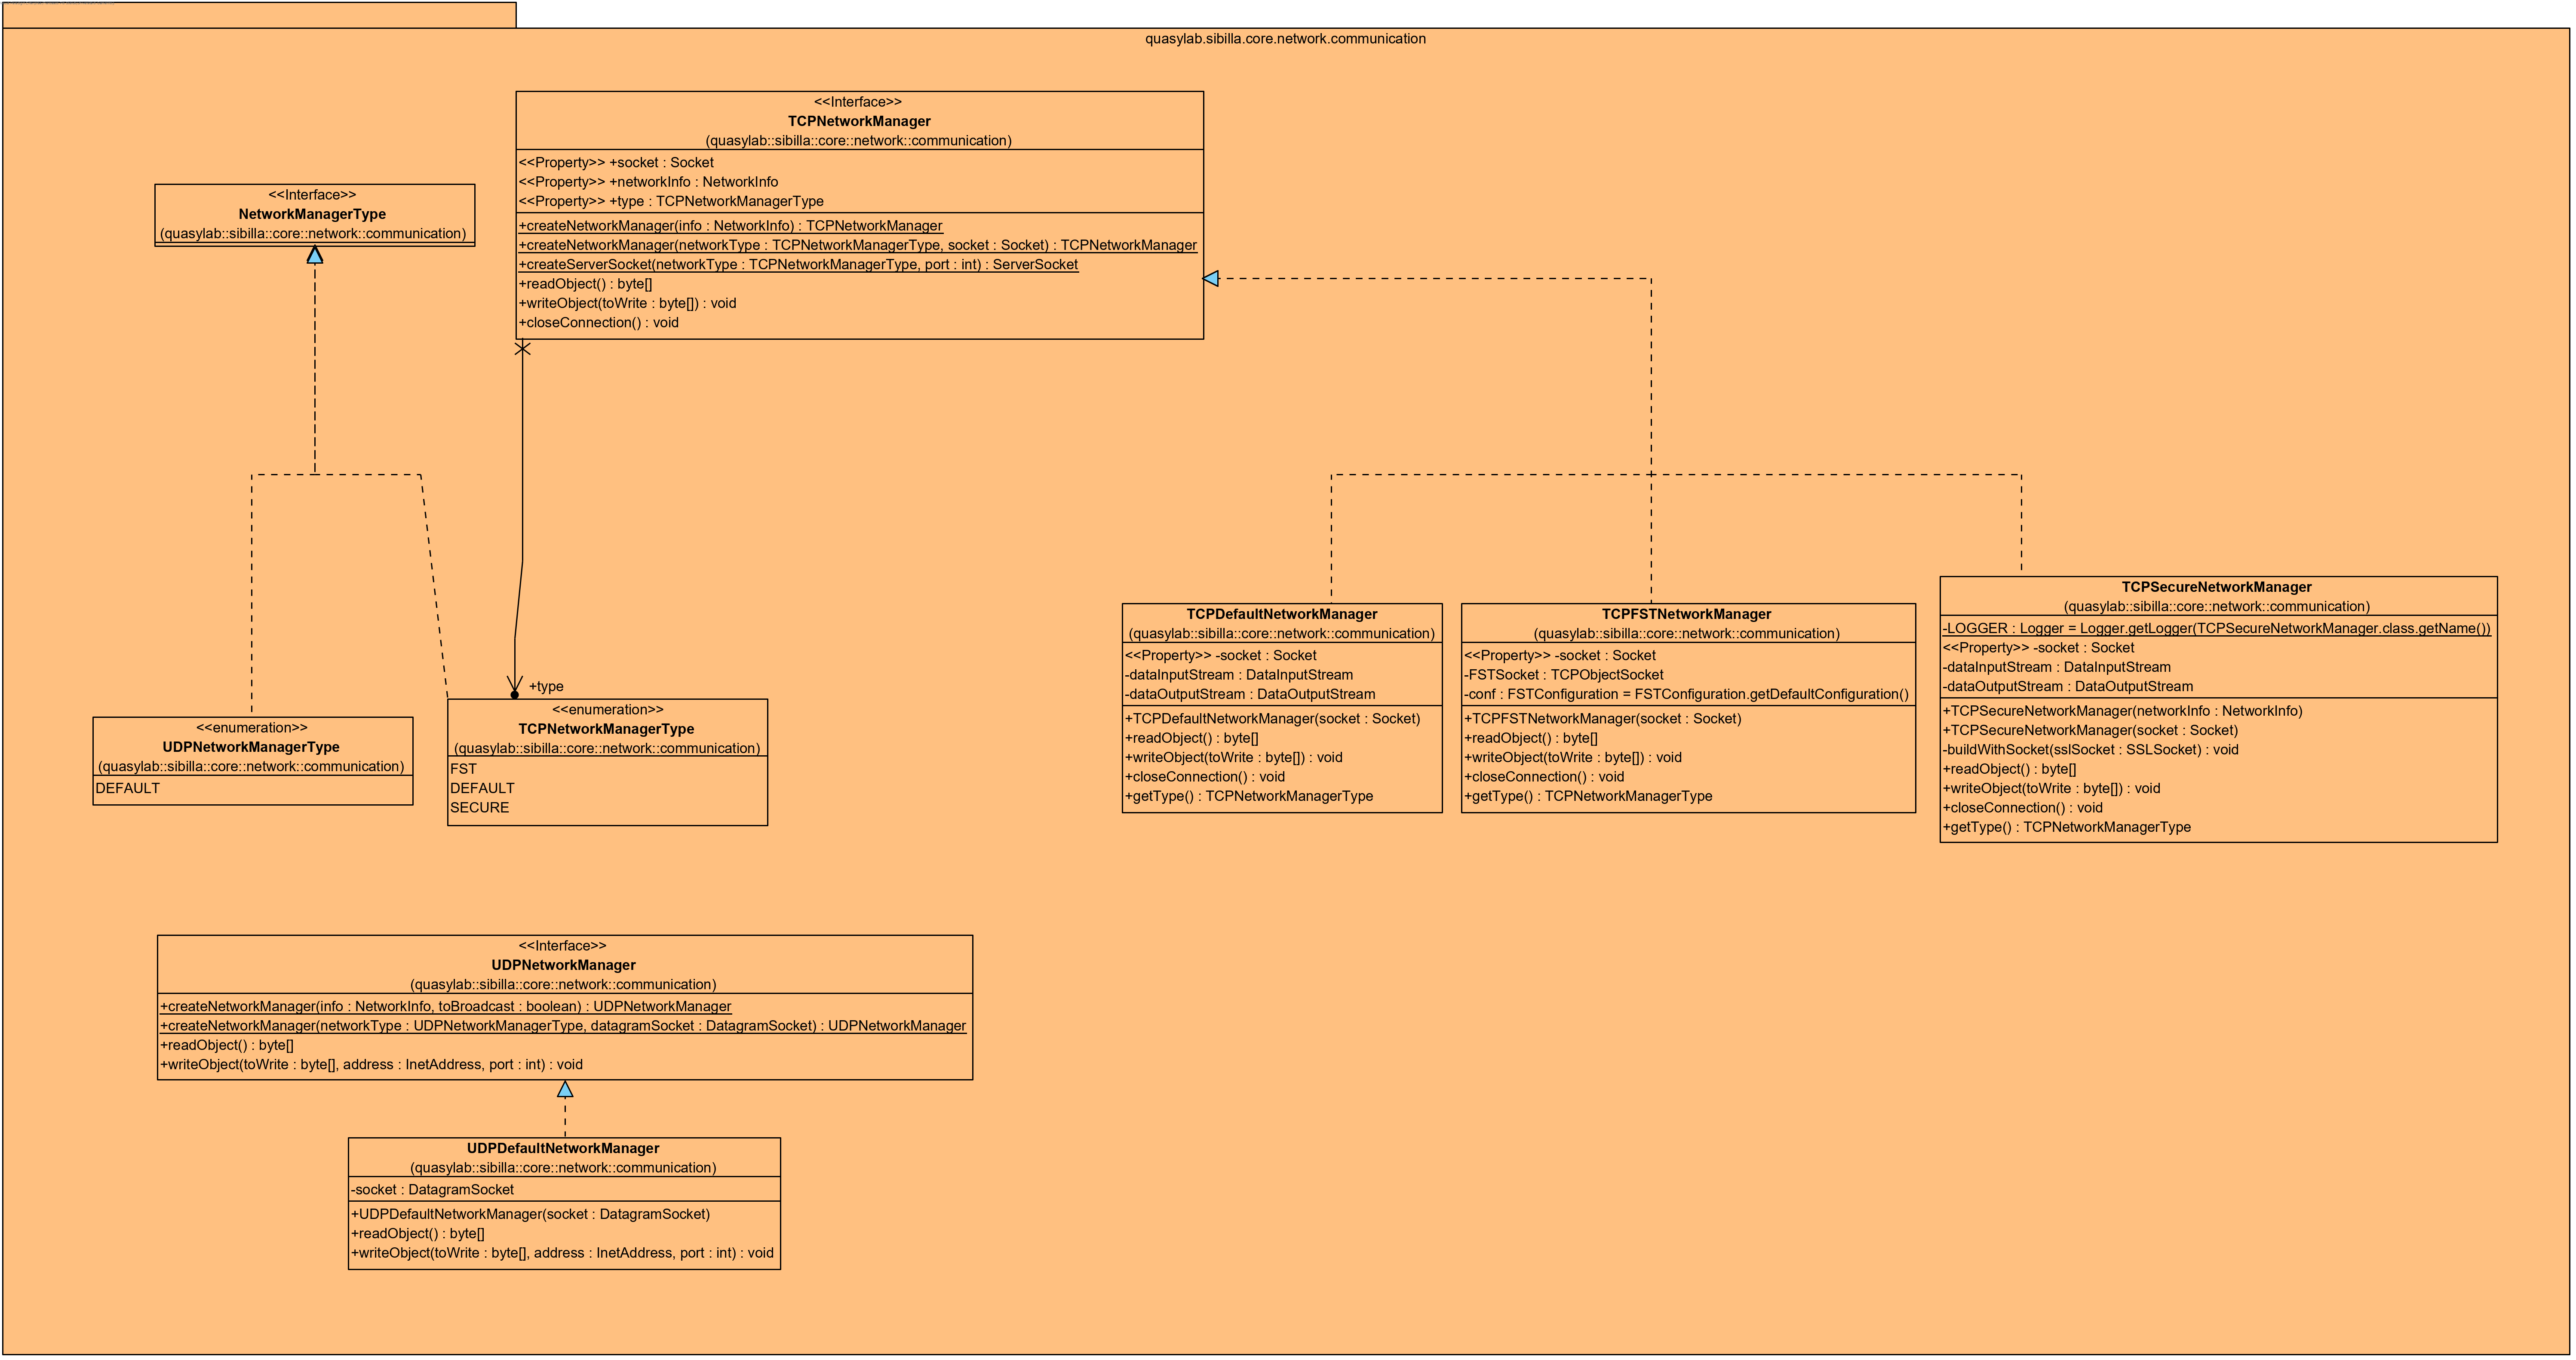
\includegraphics[width=\linewidth]{images/quasylab.sibilla.core.network.communication.png}
    \captionsetup{justification=centering}
    \caption{Diagramma delle classi del package \texttt{quasylab.sibilla.core.network.communication}}
  \end{figure}

\subsection{\texttt{quasylab.sibilla.core.network.compression}} Contiene le classi di utilità che sono impiegate per la \textbf{compressione} e la \textbf{decompressione} dei messaggi e dei dati all’interno del protocollo di comunicazione. Il funzionamento delle classi all’interno del pacchetto si basa sulla libreria \texttt{java.util.zip}.

\begin{figure}[H]
    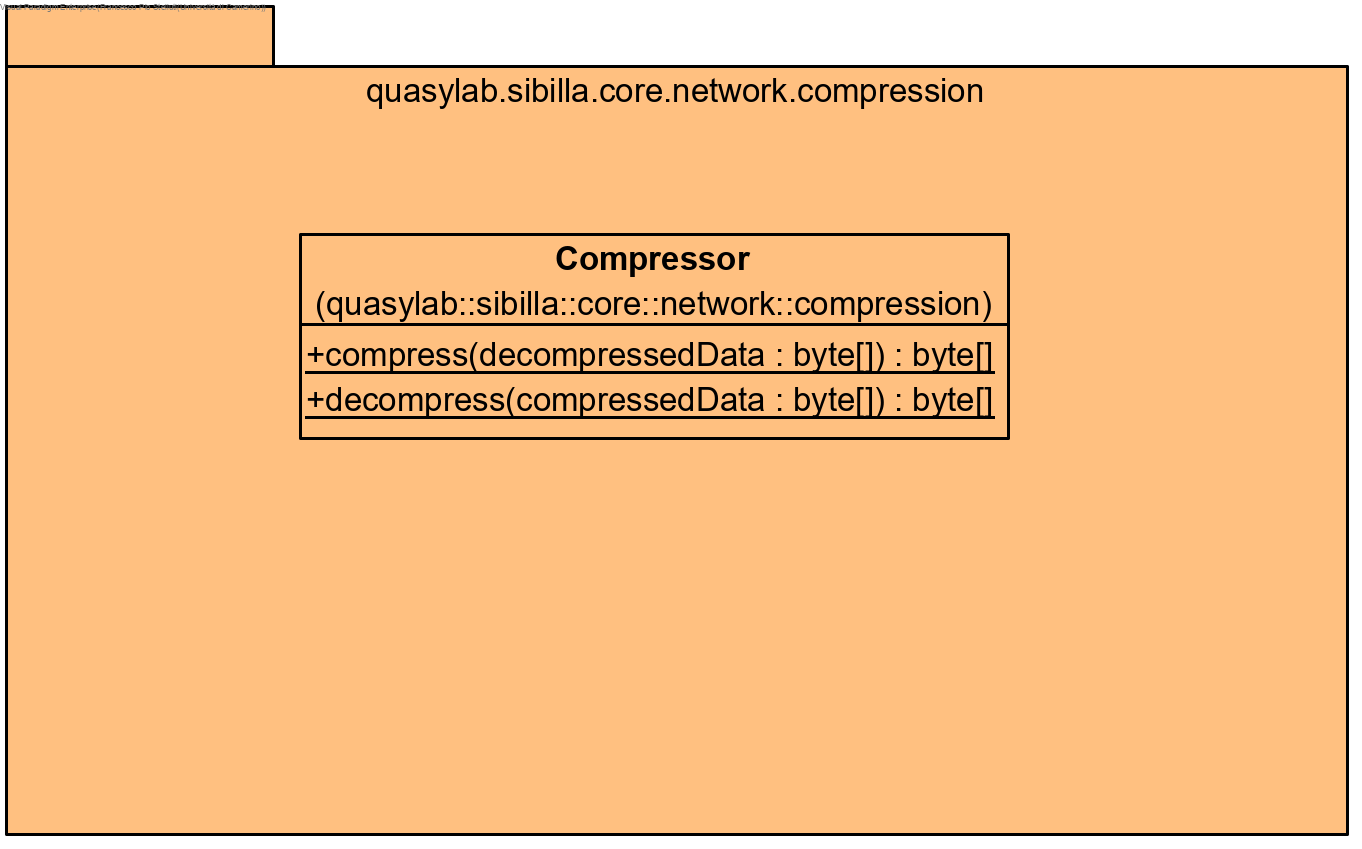
\includegraphics[width=\linewidth]{images/quasylab.sibilla.core.network.compression.png}
    \captionsetup{justification=centering}
    \caption{Diagramma delle classi del package \texttt{quasylab.sibilla.core.network.compression}}
  \end{figure}

\subsection{\texttt{quasylab.sibilla.core.network.serialization}} Contiene le classi di utilità che sono impiegate per la \textbf{serializzazione} e \textbf{deserializzazione} dei messaggi e dei dati all’interno del protocollo di comunicazione e per il \textbf{caricamento} a tempo d’esecuzione delle classi contenenti i modelli delle simulazioni da elaborare e gestire. Il funzionamento delle classi relative alla serializzazione si basa sulla libreria \texttt{org.apache.commons.lang3}.

\begin{figure}[H]
    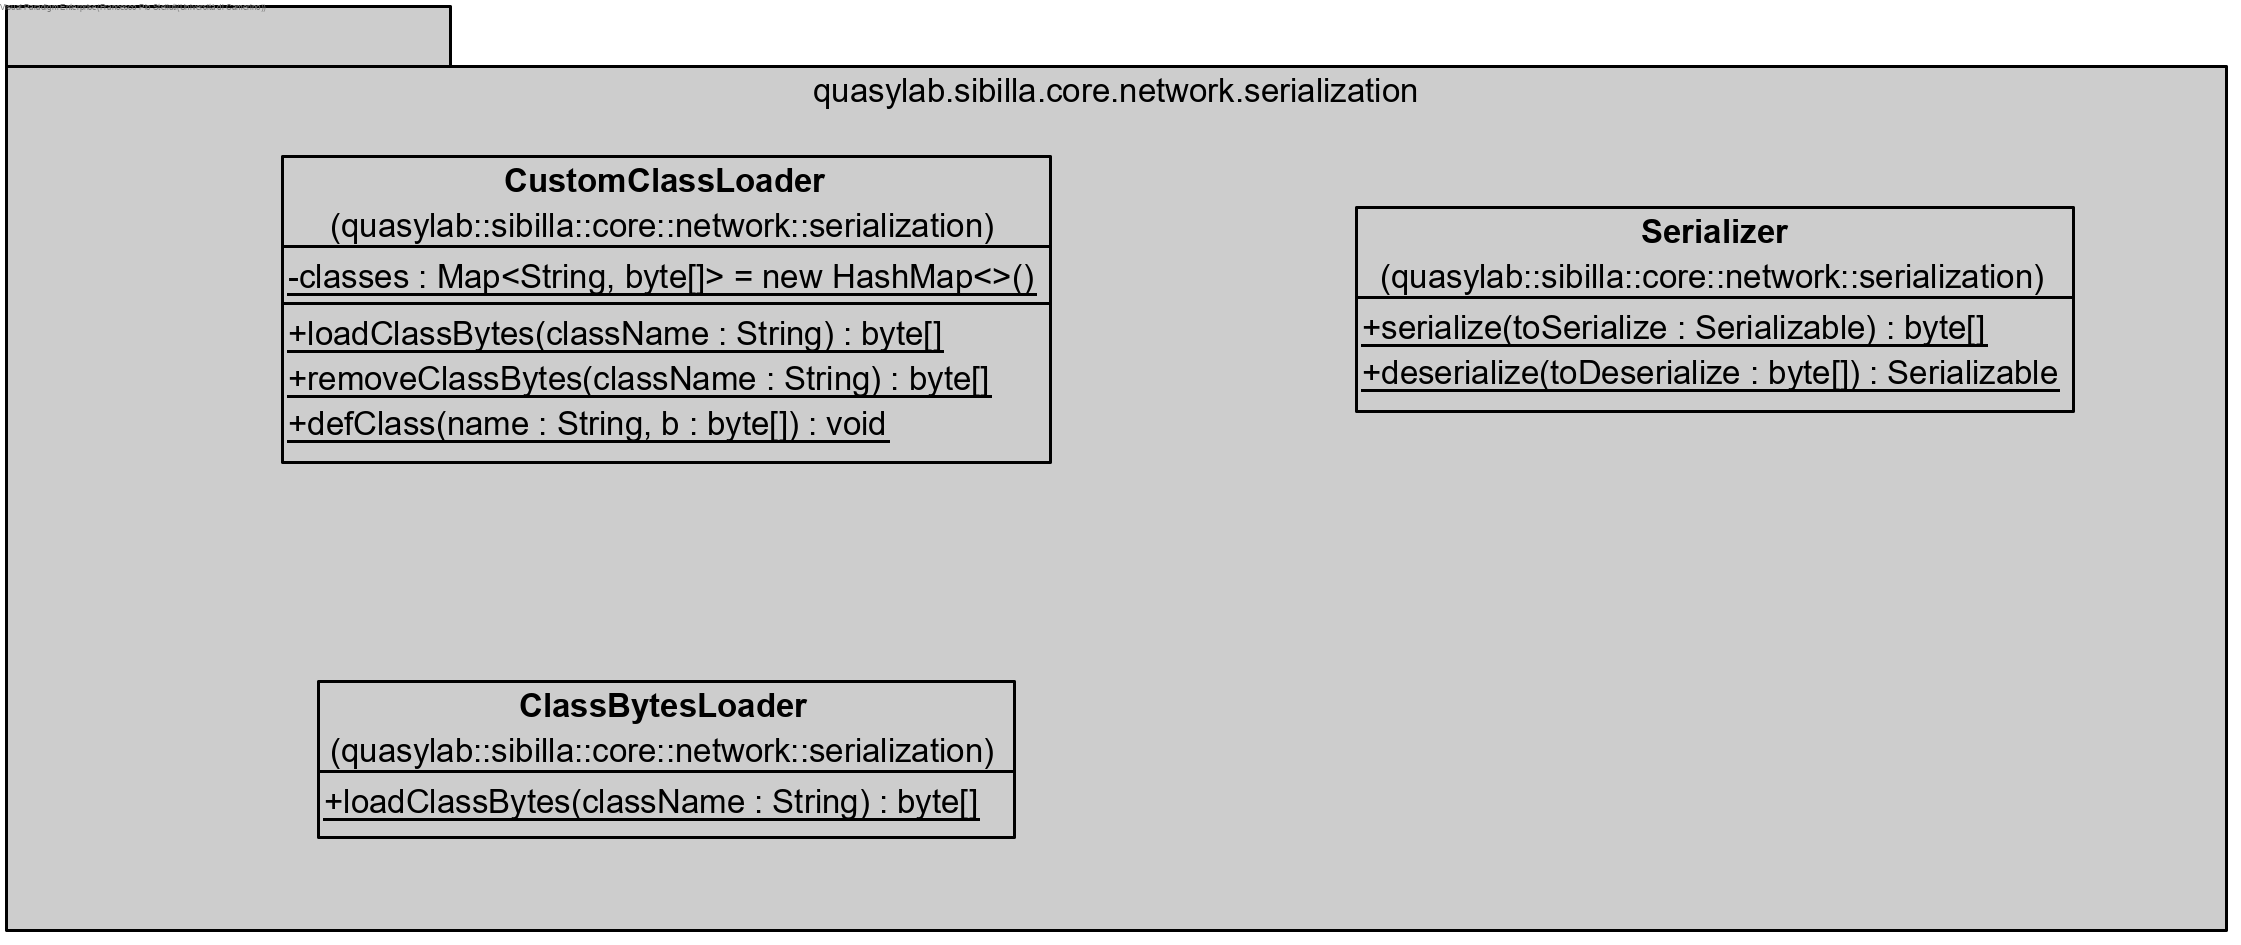
\includegraphics[width=\linewidth]{images/quasylab.sibilla.core.network.serialization.png}
    \captionsetup{justification=centering}
    \caption{Diagramma delle classi del package \texttt{quasylab.sibilla.core.network.serialization}}
  \end{figure}

\subsection{\texttt{quasylab.sibilla.core.network.util}} Contiene varie classi di utilità che sono impiegate all’interno delle classi della libreria. Tra le funzionalità di tali classi rientrano il configurare e gestire i parametri per le comunicazioni in rete basate su \textbf{SSL} o \textbf{TLS}, l’ottenere informazioni utili relative alle \textbf{interfacce di rete} del dispositivo e il configurare e gestire i \textbf{parametri di avvio} all’interno delle classi che decidono di implementare ed utilizzare le classi della libreria.

\begin{figure}[H]
    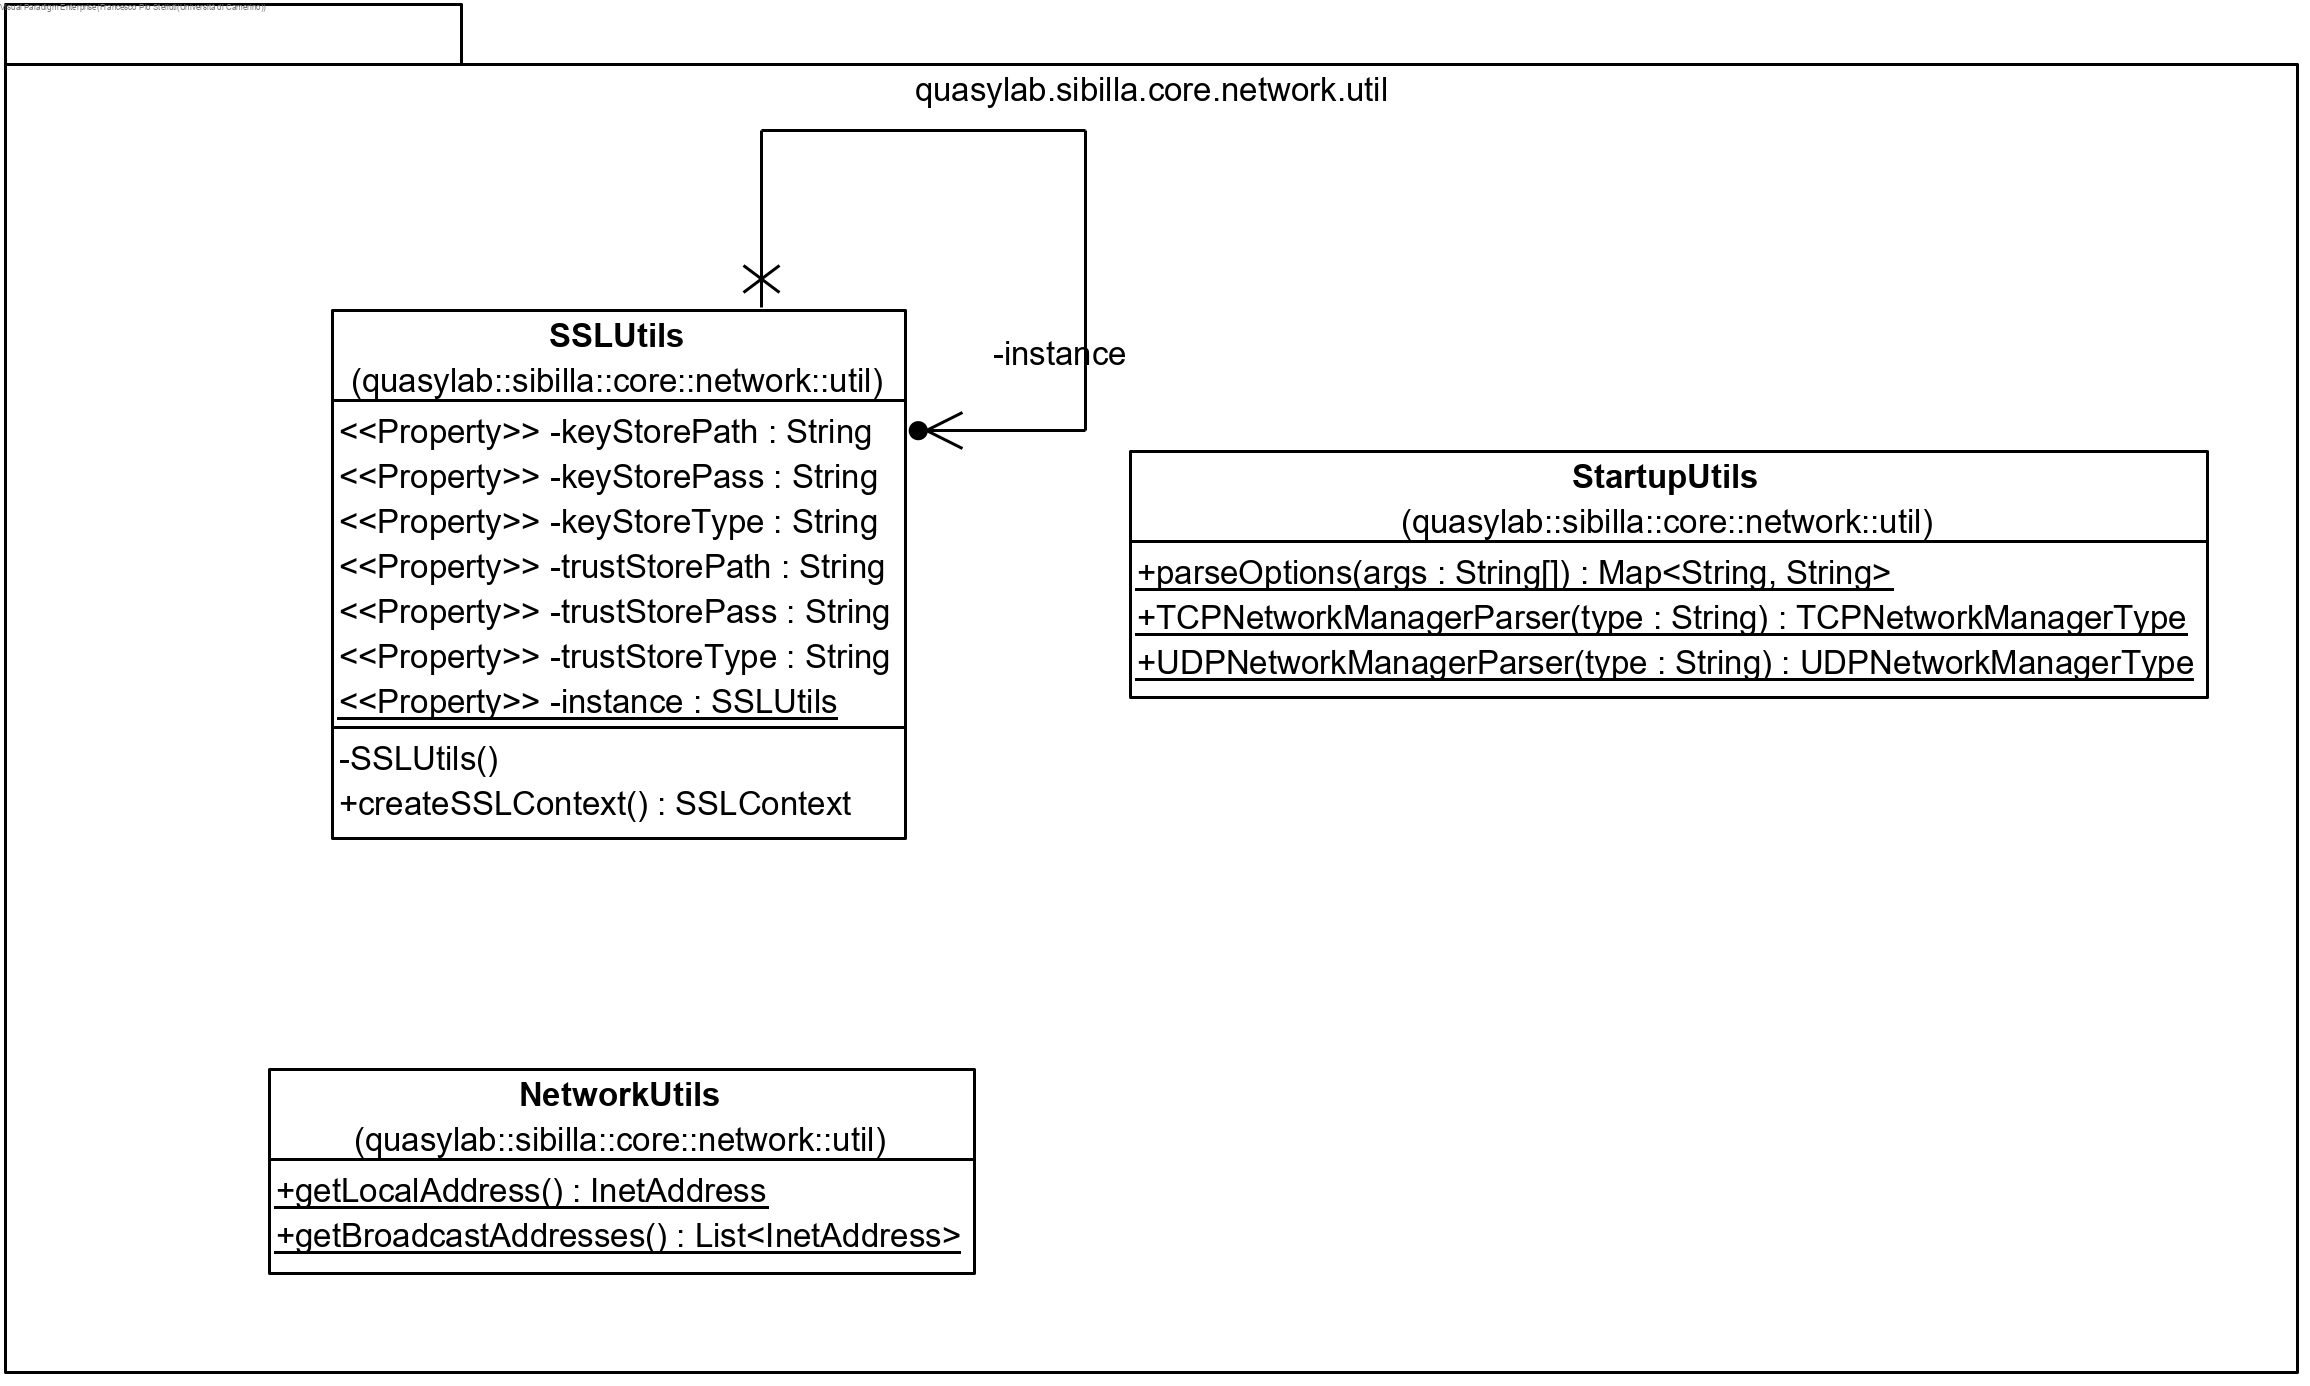
\includegraphics[width=\linewidth]{images/quasylab.sibilla.core.network.util.png}
    \captionsetup{justification=centering}
    \caption{Diagramma delle classi del package \texttt{quasylab.sibilla.core.network.util}}
  \end{figure}













